\chapter{Background}
\label{background}
\section{Deforestation and the \textit{Ley de Bosques} (Forest Act) in Argentina}

The conversion of forestland to other uses has seriously impacted Argentina’s forests. In 1915 it was remarked that 30 percent of the country had forest cover, but in 2001 only 10 percent remained forested \autocite{secretaria-de-d2001primer}. Over the period 1998 to 2002, Argentina lost over 940,000 hectares of forest cover \autocite{secretaria-de-a2007informe}. This high rate of deforestation concerned policymakers. Law 26.331, or the \textit{Ley de Bosques} (Forest Act), was passed in November 2007 in an effort to preserve remaining native forest. Areas of native forest are defined to be those with forest cover of at least 20 percent native species, and that have trees of a minimum of seven meters high. The law designates red, yellow, and green areas, each with different restrictions on clearing and use. Red is assigned to areas of ``high conservation value,'' yellow is for areas that must be managed sustainably, and green allows ``partial or total use'' \autocite[25]{gulezian2009environmental}. Each provincial government is responsible for determining how to classify their native forest areas, and each enacted the \textit{Ley de Bosques} regulations under the \textit{Ordenamiento Territorial de los Bosques Nativos} (Land Management Order for Native Forests, OTBN).

As a part of Law 26.331, ongoing land cover studies are done to examine the effectiveness of the legislation. Between 2006 and the passing of the law, 573,296 hectares of native forest cover were lost (see \cref{table:deforestationAR}). From the passing of the law in 2007 and the classification of the OTBN areas in 2009, a further 473,001 hectares were deforested. From the enacting of the OTBN (in 2009) and 2011, some 459,108 hectares were found to have been lost \autocite{secreteria-de-a2012monitoreo}. The continued deforestation suggests that, in the context of the native forest areas, the \textit{Ley de Bosques} may have had a small effect in reducing deforestation. Yet the overall deforestation rate remains quite high. Consequently, some have begun to question the effectiveness of the law at slowing cutting \autocites{valpreda2012the-protection}{greenpeace-arge2013ley-de-bosques:}. Clearly, a better understanding of the driving forces of deforestation in Argentina needs to be developed.

\begin{table}
\begin{Spacing}{1.0}
  \centering
  \caption{Deforestation in Argentina, 2006 to 2011}
  \label{table:deforestationAR}
  \begin{tabu} to 5in {X[c]X[c]}
  \toprule
  \textbf{Time Period} & \textbf{Hectares Deforested} \\
  \midrule
  2006 to Ley de Bosques (2007) & 573,296 \\
  Ley de Bosques to OTBN (2009) & 473,001 \\
  OTBN to 2011 & 459,108 \\
  \midrule
  \textbf{Total} & 1,505,405 \\
  \bottomrule
  \end{tabu}
\end{Spacing}
\end{table}


\section{Soy and its Effects}

The increase of soybean cultivation in Argentina has occurred at a rapid pace throughout the last two decades, making it the third largest producer of soy in the world \autocite{us-foreign-agri2013world}. Necessarily, as soy production rises, so does its spatial extent and the intensity of cultivation methods. Currently, almost all of Argentina’s soy production uses genetically modified (GM) varieties, specifically Monsanto’s ``Roundup Ready'' beans \autocite{greenpeace-inte2005the-expanding}. The highly mechanized and input intensive nature of this crop type calls into question other environmental consequences of soybean cultivation, such as pesticide runoff, glyphosate-resistant weeds, and soil depletion \autocite{pengue2005transgenic}. The significant capital expense for such mechanical and chemical technologies consolidates land ownership into the hands of an elite few as small famers find themselves unable to compete with larger producers' economies of scale.

A number of studies have addressed soy and deforestation in Northwest Argentina, but only one has used methods capable of mapping crop types in deforested areas \autocite{volante2005analisis}. However, this study by the Argentine \textit{Instituto Nacional de Tecnología Agropecuraia} (National Institute of Agricultural Technology, INTA) does not have well-documented methodology and has not been updated since 2005. Of the remainder, all used remote sensing techniques to classify only LULC and not specific crop types, leaving the effect of soy on LULC as an underlying assumption \autocites{grau2005agriculture}
{grau2008balancing}{grau2005globalization}
{boletta2006assessing}{gasparri2009deforestation}. While the extreme deforestation in Argentina is undeniable---and certainly soy plays a part---soy's role has not been examined in full, leaving unsubstantiated the perception of soy as the driving force in this process.

The goal of this research is to develop an image classification method capable of mapping agricultural crops by type, allowing soy to be explicitly identified on remotely sensed imagery. Accurate and efficient mapping of soy distributions and their changes over time will allow further investigation of the roles of soy in deforestation. The direct and indirect effects soy crops have had on deforestation can thus be understood conceptually and systemically at both regional and local scales, which could lead to the development of more effective policies for land management \autocite{brown2007multitemporal}.


\section{Composite Vegetation Indices and Time-Series Images}

The differentiation of crop types in remotely-sensed imagery is not a straightforward process. The use of a vegetation index (VI), such as the normalized difference vegetation index (NDVI) or the enhanced vegetation index (EVI), can help identify crops by their specific VI values in an image.

NDVI is a normalized ratio of the red and near-infrared bands, and can be expressed mathematically as:
\begin{equation}
  NDVI = \frac{\rho~_{NIR} - \rho~_{red}}{\rho~_{NIR} + \rho~_{red}}
\end{equation}
where $\rho~_{NIR}$ and $\rho~_{red}$ are the measured surface reflectance in their respective bands. As a ratio, the index minimizes multiplicative noise, but has issues with non-linearity and additive noise \autocite{huete2002overview}.

With advances in calibration, atmospheric correction, and other noise removal techniques, which are integrated into the MODIS data processing workflow, a ratioing index is less necessary. The EVI was specifically developed for the MODIS platform to help correct some of the deficiencies of the NDVI. It has better sensitivity to high biomass, canopy structure, and leaf area, and less susceptibility to atmospheric degradation. EVI is calculated as:
\begin{equation}
  EVI = G\frac{\rho~_{NIR} - \rho~_{red}}{\rho~_{NIR} +  C_1\times\rho~_{red} - C_2 \times \rho~_{blue} + L}
\end{equation}
Again, each $\rho$ is the measured surface reflectance in the respective band, after complete or partial atmospheric correction. The blue band is used to ``subtract'' aerosol effects from the red band. Additionally, four coefficients are introduced: $G$ is the gain factor, $C_1$ and $C_2$ are used in the aerosol calculation, while $L$ ``is the canopy background adjustment that addresses nonlinear, differential NIR and red radiant transfer through a canopy'' \citereset\autocite[196]{huete2002overview}. The values of these coefficients as used in the MODIS EVI calculation are 2.5, 6.0, 7.5, and 1.0, respectively.

Some crops, such as soy and sugarcane, have very different spectral reflectance throughout their development and maturation. However others, such as soy and corn, can have very similar spectral reflectance, leading to overlapping VI ranges \autocite{price1994how-unique}. Such overlap can make it impossible to determine a crop type with specificity using traditional approaches; even using hyperspectral data, few differentiating characteristics between crops can hinder classification. To combat this ambiguity, imagery from multiple dates can be used to show VI values over time, allowing the development of a classifier based on crop phenologies rather than reflectance values on a single-date \autocites{gu2010phenological}{wardlow2002discriminating}{wardlow2005state-level}{wardlow2007analysis}{wardlow2008large-area}{zhang2003monitoring}. \autoref{fig:tsi} shows an example of how the VI values change over a growing season.

\begin{ssfigure}
  \centering
  \begin{subfigure}[t]{\textwidth}
    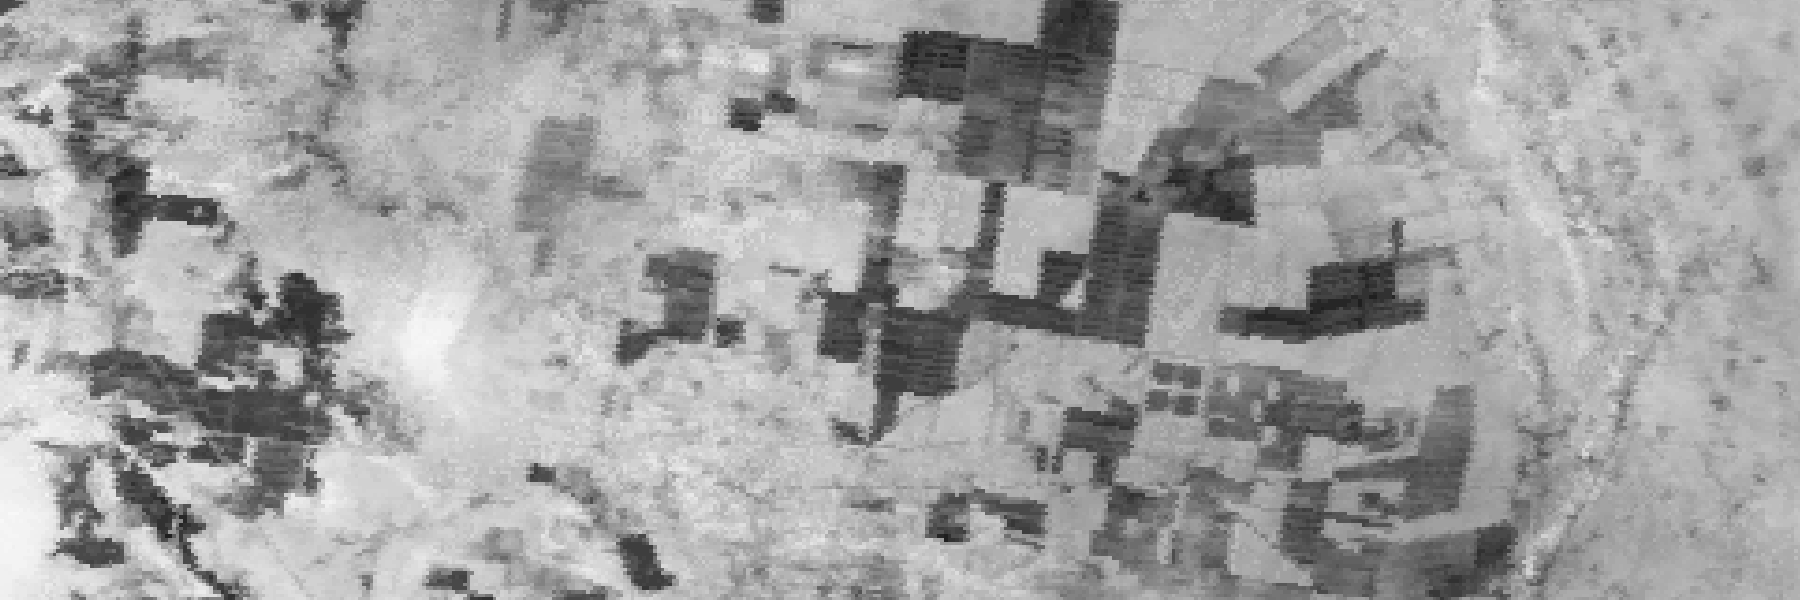
\includegraphics[width=\textwidth]{Graphics/vi_band1.png}
    \caption*{\formatdate{19}{12}{2013}}
    \label{subfig:vi_1}
  \end{subfigure}
  \\
  \vspace{0.125in}
  \begin{subfigure}[t]{\textwidth}
    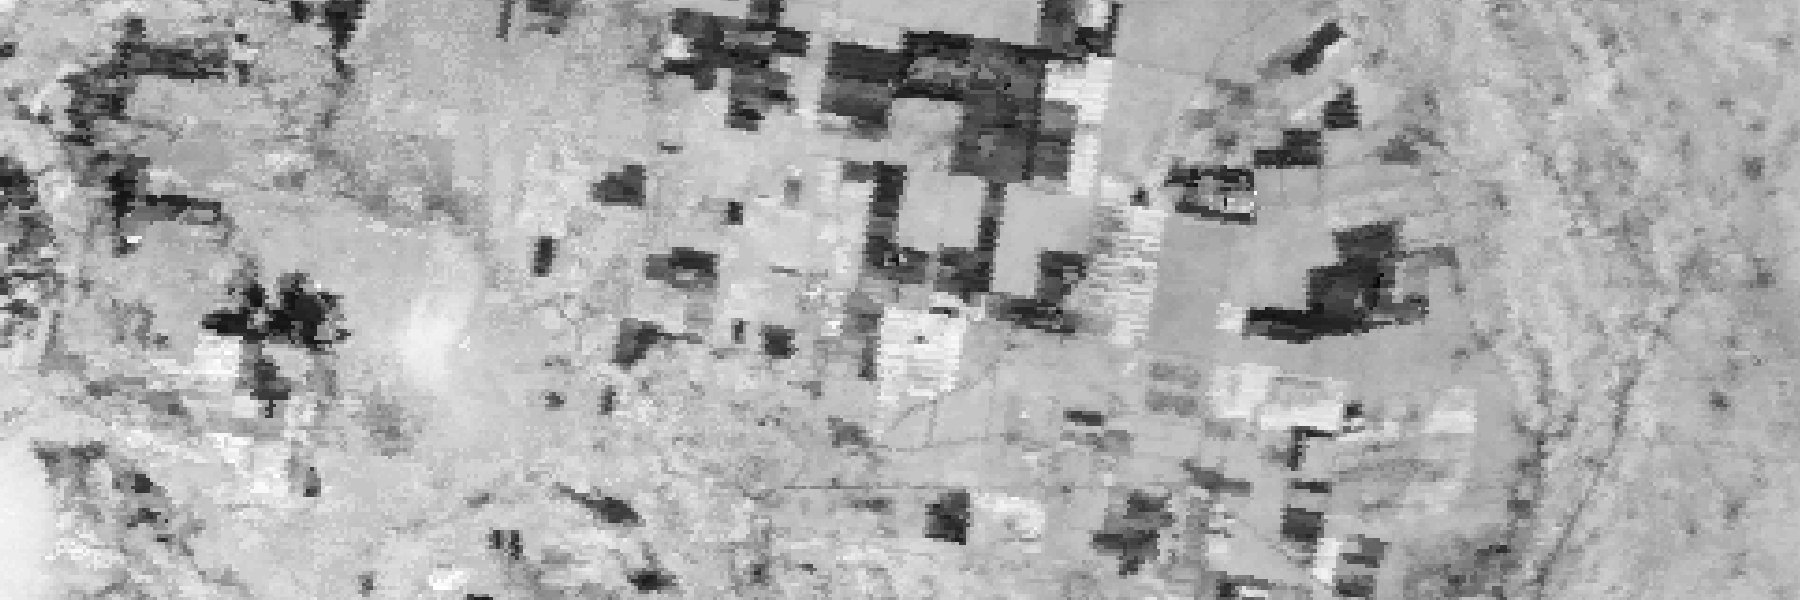
\includegraphics[width=\textwidth]{Graphics/vi_band4.png}
    \caption*{\formatdate{2}{2}{2014}}
    \label{subfig:vi_4}
  \end{subfigure}
  \\
  \vspace{.125in}
  \begin{subfigure}[b]{\textwidth}
    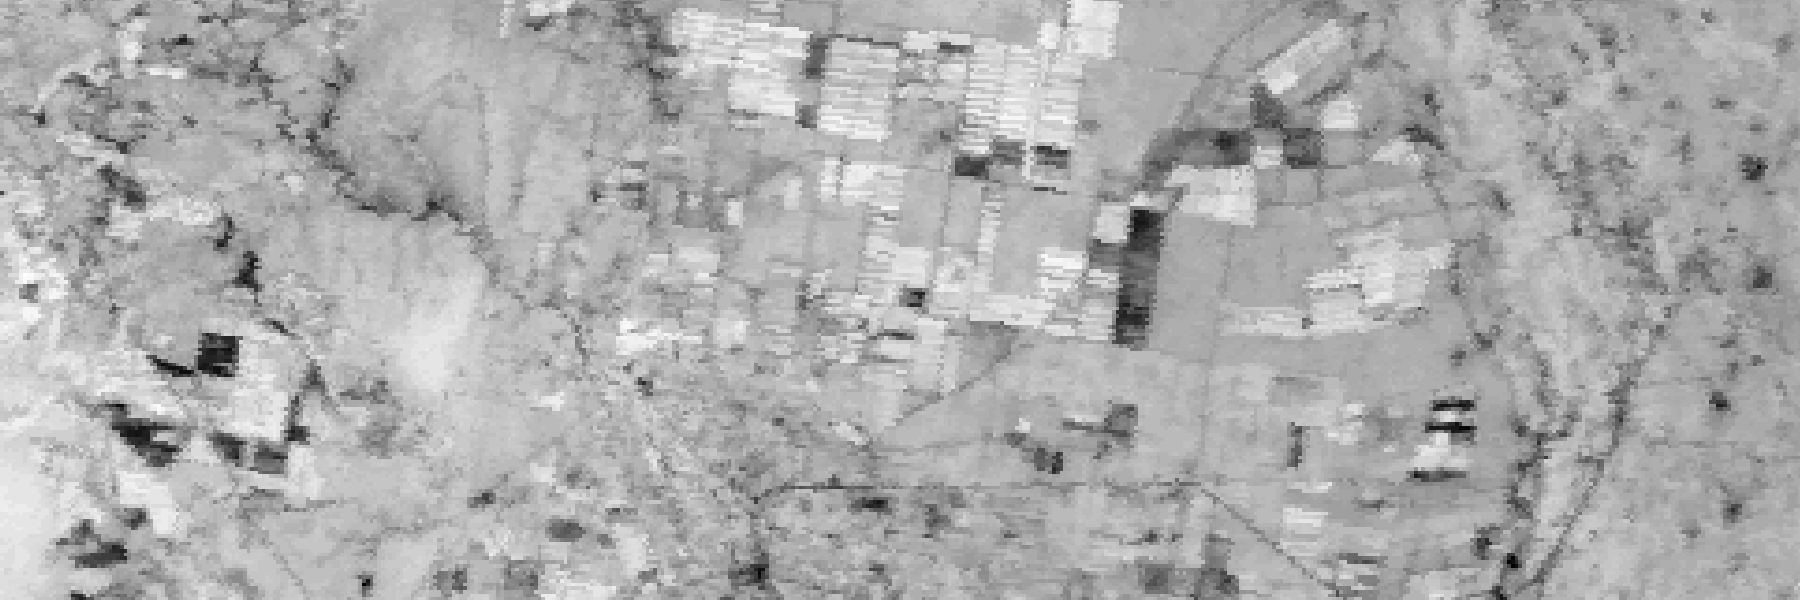
\includegraphics[width=\textwidth]{Graphics/vi_band8.png}
    \caption*{\formatdate{7}{4}{2014}}
    \label{subfig:vi_8}
  \end{subfigure}
  \caption{Example VI Progression}
  \label{fig:tsi}
  \medskip
  \small
  These MODIS NDVI images show the progression of VI values for a section of a MODIS tile containing the north half of Pellegrini and the surrounding area. The relatively constant medium-gray values for the forested areas stand in stark contrast to the fields, which predominately begin with low VI values (dark) in the first image, increasing as the crops mature to the greater VI values (bright) shown in the last image.
\end{ssfigure}
	
MODIS 16-day VI composite imagery from both the Terra and Aqua Earth Observing System (EOS) satellites is available from the Land Processes Distributed Active Archive Center (LPDAAC).\footnote{For those interested in working with MODIS data, the web address of LPDAAC is https://lpdaac.usgs.gov/, though data are not directly available from their servers without an exact link. I found the best tool for searching the available data was NASA’s Reverb|Echo web tool, at https://reverb.echo.nasa.gov/. Using this tool, one can get a list of links in a text file, and can use wget or curl to bulk download the files in the list.} Each MODIS satellite images the entire Earth daily: the Terra satellite makes its passes north to south, while Aqua orbits south to north. Both cross the equator at noon. The daily temporal resolution is the greatest advantage of the MODIS platform. The likelihood of getting enough cloud-free data to develop a phenologic model is significantly increased over other common platforms like Landsat Thematic Mapper (TM) and Landsat Operational Land Imager (OLI), which have repeat coverage only every sixteen days. MODIS data, however, comes at the price of reduced spatial resolution: 231 meters compared to Landsat’s 30-meter pixels.\footnote{Though the literature typically denotes MODIS data as 250-meter, the composite vegetation indices are actually 231-meter. However, to stay consistent with conventions, I will refer to the data as 250-meter.} At this resolution, crop mapping is restricted to medium farms and larger---those with fields of at least 231 meters square, though often a field must be up to two times larger in at least one dimension to ensure a pure pixel can be isolated. For the purposes of this investigation, however, this limitation is inconsequential, as small farms have a relatively minor impact on deforestation due to their size. Moreover, the crop of interest, GM soy, is only profitably grown using highly mechanized, input-intensive agricultural practices at very large scales \autocite{kaimowitz2001soybean}. Small fields do not have high enough yields to overcome the significant capital investment required.

LPDAAC creates the VI composites using the maximum VI value over the proceeding 16-day time period. Clouds, which have low VI values, are often eliminated completely over this composite period. The images are numbered by the day of the year (DOY) of the last date in the image's date range, so an image from DOY 17 is the composite of the images from \datenoyear{1}{1} through \datenoyear{17}{1}.\footnote{Following this pattern exactly will make the first image from the following year be from \datenoyear{4}{1}, but the MODIS composite numbering ``resets'' at the end of each year. Thus the image interval at the end of the year is shortened, allowing the next image to be produced \datenoyear{1}{1}, though it still covers the proceeding 16 days.} Both NDVI and EVI are included in the MODIS VI products, and require no preprocessing for immediate use (unless cloud cover is pervasive in the area). A chronological series of these VIs can be assembled into a time series image (TSI), which can then be used for processing.


\section{Crop Phenologies and Phenological Classification}
\label{methods:phenology-fitting}

\citeauthor{gu2010phenological} outlined that phenological statistics regarding vegetation development can be derived from a MODIS VI time-series, including ``start-of-season time, start-of-season NDVI, end-of-season time, end-of-season NDVI, maximum NDVI, maximum NDVI time, duration of season, amplitude of NDVI, and seasonal time integrated NDVI'' \mkbibparens{\citeyear[529]{gu2010phenological}}. A principal component analysis can then be used to extract the meaningful variation in the data.

Similarly, Wardlow, Egbert, et al. \autocites{wardlow2002discriminating}{wardlow2005state-level}{wardlow2007analysis}{wardlow2008large-area} showed that a decision tree classifier can be used to classify vegetation time-series data into increasingly refined categories until specific crop types are isolated and classified. Beginning with a basic land cover classification (e.g. forest, urban, agriculture), crops in the agriculture class are broken down into winter and summer varieties using peaks in the vegetation index (winter wheat will peak earlier in the year than summer crops like corn and soy). Then, using training sites of known crop types defined by ground truth data, a final crop classification can be assigned by finding pixel values for key dates where like crops can be differentiated. That is, using the growing season in the Northern Hemisphere as an example, if from the training sites we know summer crop A has VI values between 0.7 and 0.8 on \datenoyear{26}{6} and between 0.5 and 0.6 on \datenoyear{29}{8}, while summer crop B is between 0.55 and 0.65 and 0.75 and 0.85 on the same dates, pixels in the summer crop class can be assigned one of these types by testing their pixel values on these dates. The authors found this method to have about an 85 percent overall accuracy \autocite{wardlow2005state-level}. However, this method requires training sites with previously-determined crop types to produce a classification, which can be time consuming and expensive to acquire.

\textcite{masialeti2010a-comparative} found that VI values from one year have a significant correlation with values from other years. They compared the phenological curves of crops formed by the NDVI values from 2001 MODIS data \autocite[from][]{wardlow2005state-level} with those from 2005 MODIS data. Generally, the shape of each crop's curve is maintained year-to-year, but three subtle transformations may occur depending on weather and other external variables: (1) a shift in the beginning of the curve (earlier or later planting), (2) a scaling of the maximum of the curve (better or worse crop development), and (3) a scaling of the spread of the curve (a longer or shorter growing season) (\autoref{fig:transformations}). They surmised, with a means to account for the shift and scaling of the curve, one could use VI values from one year to classify those from another.

\begin{ssfigure}
  \centering
  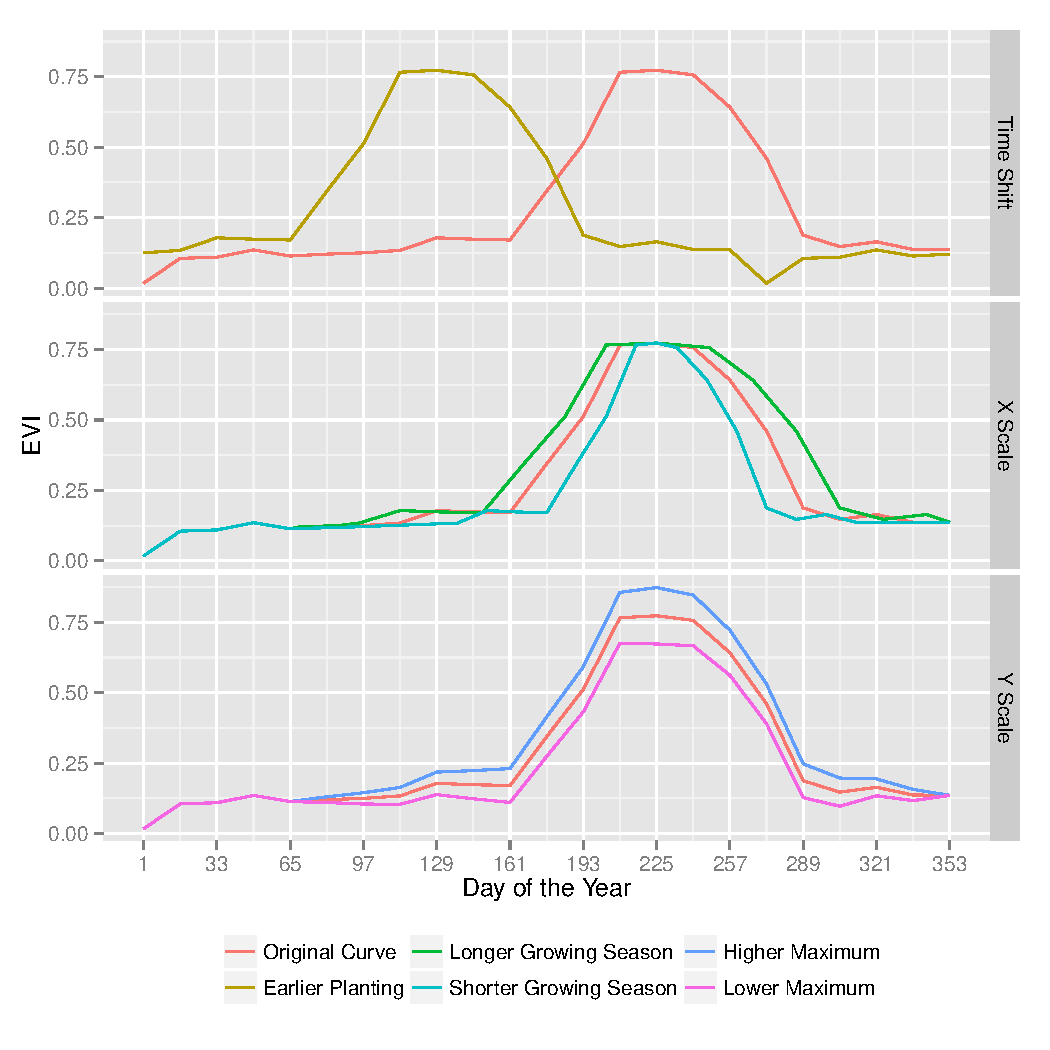
\includegraphics[width=\textwidth]{Graphics/transformations.pdf}
  \caption{Example Transformations of a Crop's VI Curve}
  \medskip
  \small
  The original signature was derived from soy in southwestern Kansas. The other signatures were arbitrarily adjusted to illustrate each of the possible transformations (the diagrams were created for illustration purposes).
  \label{fig:transformations}
\end{ssfigure}

Even without a mechanism to account for interannual differences, \textcite{brown2007multitemporal} used crop phenologies derived from multiple years of data to test four phenological classification methods. The authors fit the known phenologies to unknown phenologies from other years by comparing the VI values throughout the growing season. The degree of likeness between a known VI curve and the unknown VI curve determined the classification. They showed that the best of the four classification methods tested was to find the sum of the square errors between the known and unknown curves (the SSE method, \citeauthor{brown2007multitemporal} pg. 131).

The similarities between the methods presented by \citeauthor{brown2007multitemporal} and hyperspectral remote sensing techniques are striking. Hyperspectral techniques compare known \textit{spectral signatures} from a signature library to the unknown pixel signatures in an image. One method, spectral feature fitting, uses a least-squares comparison reminiscent of SSE from \citeauthor{brown2007multitemporal} \autocites{solutions2013selected}{clark2003imaging}. The key difference between the two, besides comparing reflectance across time versus reflectance across the electromagnetic spectrum, is that spectral feature fitting does not require any training data from the processed image. All of the spectral signatures used for identification are from standardized spectral libraries, which contain the many spectra of different materials.

Accordingly, one goal of this study is to realize a method of vegetation classification using multi- or hyper-temporal imagery that does not require training data to be extracted from the imagery itself. The method would use standard libraries of phenological curves---\textit{temporal signatures}---for different vegetation and non-vegetation land covers. A major challenge of this idea is that, unlike spectral signatures, temporal signatures are not necessarily consistent location to location nor year to year, as mentioned by \citeauthor{masialeti2010a-comparative}. A viable classification method thus must provide a way to transform the temporal signatures, within appropriate bounds, to match the horizontal scaling, vertical scaling, and time shifting of an unknown pixel before finding the degree of fit between the signature curve and the pixel curve.

\textcites{sakamoto2005a-crop}{sakamoto2010a-two-step} demonstrates a method using MODIS time-series data for use in finding key dates in a crop’s phenology, enabling better crop management strategies. Specifically, the authors’ two-step filter (TSF) method uses a wavelet transformation and a constrained minimization function to find a reference signature for a specific crop’s phenological development, and then fits that signature to known pixels of that crop type, finding the scaled dates of key transitions between developmental stages in the plants’ growth. This TSF method demonstrates that reference signatures can be fit to a pixel’s signature using a minimization function, accounting for the variations from the reference curve and the pixel curve.  This minimization method provides the means to account for the scaling and time shift differences, allowing previously-known temporal signatures (e.g. not from training sites) to be fit to unknown pixel signatures in a TSI.

Specifically, from page 2151 of \textcite{sakamoto2010a-two-step}:
\begin{equation}
\label{eq:1}
  RMSE = \biggl[\frac{1}{n}\sum_{x\ =\ j(1),\ j(2)\ldots}^{n}\bigl(f\left(x\right)-g\left(x\right)\bigr)^{2}\biggr]^{\frac{1}{2}}
\end{equation}
where $n$ is the number of dates in the TSI, $f(x)$ is the temporal signature for a given pixel in a dataset, and $x$ is the DOY, as defined by $j(y)$:
\begin{subequations}
\label{eq:DOYcalc}
  \begin{align}
    j\left(~y\right) &= k\bigl(~i\cdot~s\left(~y - 1\right)\bigr) \label{eq:jofy}\\
    \text{where\ \ \ \ } k\left(~z\right) &=
    \begin{cases}
      z, & \mbox{if } z \leq 0\\
      z - \bigl(\left(z\bmod~365\right)\bmod~i-1\bigr), & \mbox{if } z > 0
    \end{cases}
    \label{eq:kofz}
  \end{align}
\end{subequations}
such that $s$ is the interval of the imagery and $d$ is the starting date of the imagery. $g(x)$ in \autoref{eq:1} is given by:
\begin{equation}
\label{eq:gofx}
  g(x) = yscale\times~h\left(xscale\times(x + tshift)\right)
\end{equation}

Here, $x$ again is the DOY, $yscale$ and  $xscale$ are coefficients controlling the vertical and horizontal scaling of a reference signature $h(x)$, and $tshift$ is a constant representing the horizontal shift, in days, of $h(x)$. In other words, $yscale$ adjusts the reference signature to match the growth condition (i.e. maximum VI value) of the pixel (again, given by $f(x)$); $xscale$ adjusts the reference signature to match the pixel's growth cycle duration; and $tshift$, or time-shift, is the offset, in days, between the peak date of the reference signature and the peak date the pixel (see \autoref{fig:transformations}). Thus, if we minimize \autoref{eq:1} bounding $yscale$, $xscale$, and $tshift$  in $g(x)$ with reasonable values for each, we can calculate how well a given reference temporal signature $h(x)$ can be made to fit the pixel signature $f(x)$. Comparing a pixel's RMSE value from each of the reference signatures allows final classification; the signature with the lowest RMSE value has the best fit, and, of the tested signatures, provides the most probable identification.

